\section{Introduction}

A memory contract should answer four questions: which output is preserved,
relative to which reference state, by which numerical path, and across which
updates. A cache can shrink without answering them, and a fact can stop being
recalled while its influence remains in state. Dense caches and recurrent
memories can be effective, but an undifferentiated dense state does not
ordinarily expose an entry-level zero-contribution certificate or a deletion
path tied to an explicit retained-data refit.

Support Vector Attention (SV-Attention) exposes both through the active-set
geometry of a one-class support vector description~\citep{ocsvm,svdd}. Its
test-time gate partitions context keys into positive-coefficient support and
zero-coefficient reserve sets, and its readout uses those coefficients
directly. This structure yields two auditable contracts. Reserve removal
preserves the currently solved readout without re-solving
(Proposition~\ref{prop:reserve}); active-token decrement targets a retained-key
refit at the same primitive box parameter \(C\)
(Proposition~\ref{prop:decrement}).

The corresponding audit is coverage-first and quantitative. Across \(1{,}200\)
fp64 decrement/refit trials on Gaussian, redundant, real MIMIC-IV, and learned
keys, \(1{,}199\) complete. Regime-level median finite-probe
decision-function deviations range from \(4.5\times10^{-13}\) to
\(5.7\times10^{-7}\), and reference-run median deletion/refit speedups are
\(24\)--\(223\times\) on the reference CPU. The one uncovered margin-empty
path remains in the denominator.

The reserve result also has a sharp boundary. Example~\ref{ex:future} gives a
deterministic future admission that activates an earlier reserve point.
Consequently, current reserve status alone cannot certify a never-pruned
full-history trajectory (Proposition~\ref{prop:not-future}). This
theorem--counterexample pair characterizes what the gate proves now and what a
stronger streaming certificate would still need.

Verification and training use deliberately separate numerical paths. A
maintained fp64 active-set solver supports decrement and inverse reuse; a
batched FISTA/ridged-KKT path supports end-to-end training. Keeping the paths
separate is a reusable design pattern: each claim names the arithmetic that
earns it rather than transferring guarantees between implementations.
Table~\ref{tab:contract} renders these boundaries as a contract card.

Our contributions are:

\begin{enumerate}
\item \textbf{A two-sided characterization of reserve removal.} We prove the
point-in-time certificate and prove, by construction, that reserve status alone
does not guarantee full-history equivalence for every future admission
sequence.
\item \textbf{A measured fixed-\(C\) deletion contract.} We name the retained
refit target and report \(1{,}199/1{,}200\) numerical coverage alongside
completed-trial median, mean, and worst deviations.
\item \textbf{A verification/training separation.} The maintained path supplies
decrement and a custom inverse-reusing backward; the batched path supplies
parallel trainability. The contract card makes their non-transferable claims
explicit.
\item \textbf{A regime map for selection.} At matched budgets, held-out
rare-group query recall is \(0.861\) versus \(0.319\) for an oracle H2O-style
selector under skewed redundancy, and a declared same-channel ICU probe retains
\(0.80\) versus \(0.05\) of threshold hours.
A held-out-channel control retains SpO\(_2\)-threshold hours at \(0.464\)
versus \(0.225\) with SpO\(_2\) excluded from all selector inputs. A gate-off
control isolates selection, while a seven-seed language-model result
(\(p=0.001\)) establishes small-scale trainability.
\end{enumerate}

\paragraph{Scope.}
The certificates concern the solved context and a fixed-\(C\) retained-key
reference. They do not establish future-safe pruning under arbitrary
admissions or general quality and throughput superiority; downstream controls
and larger fixed-budget runs locate those open boundaries.

\begin{figure}[t]
\centering
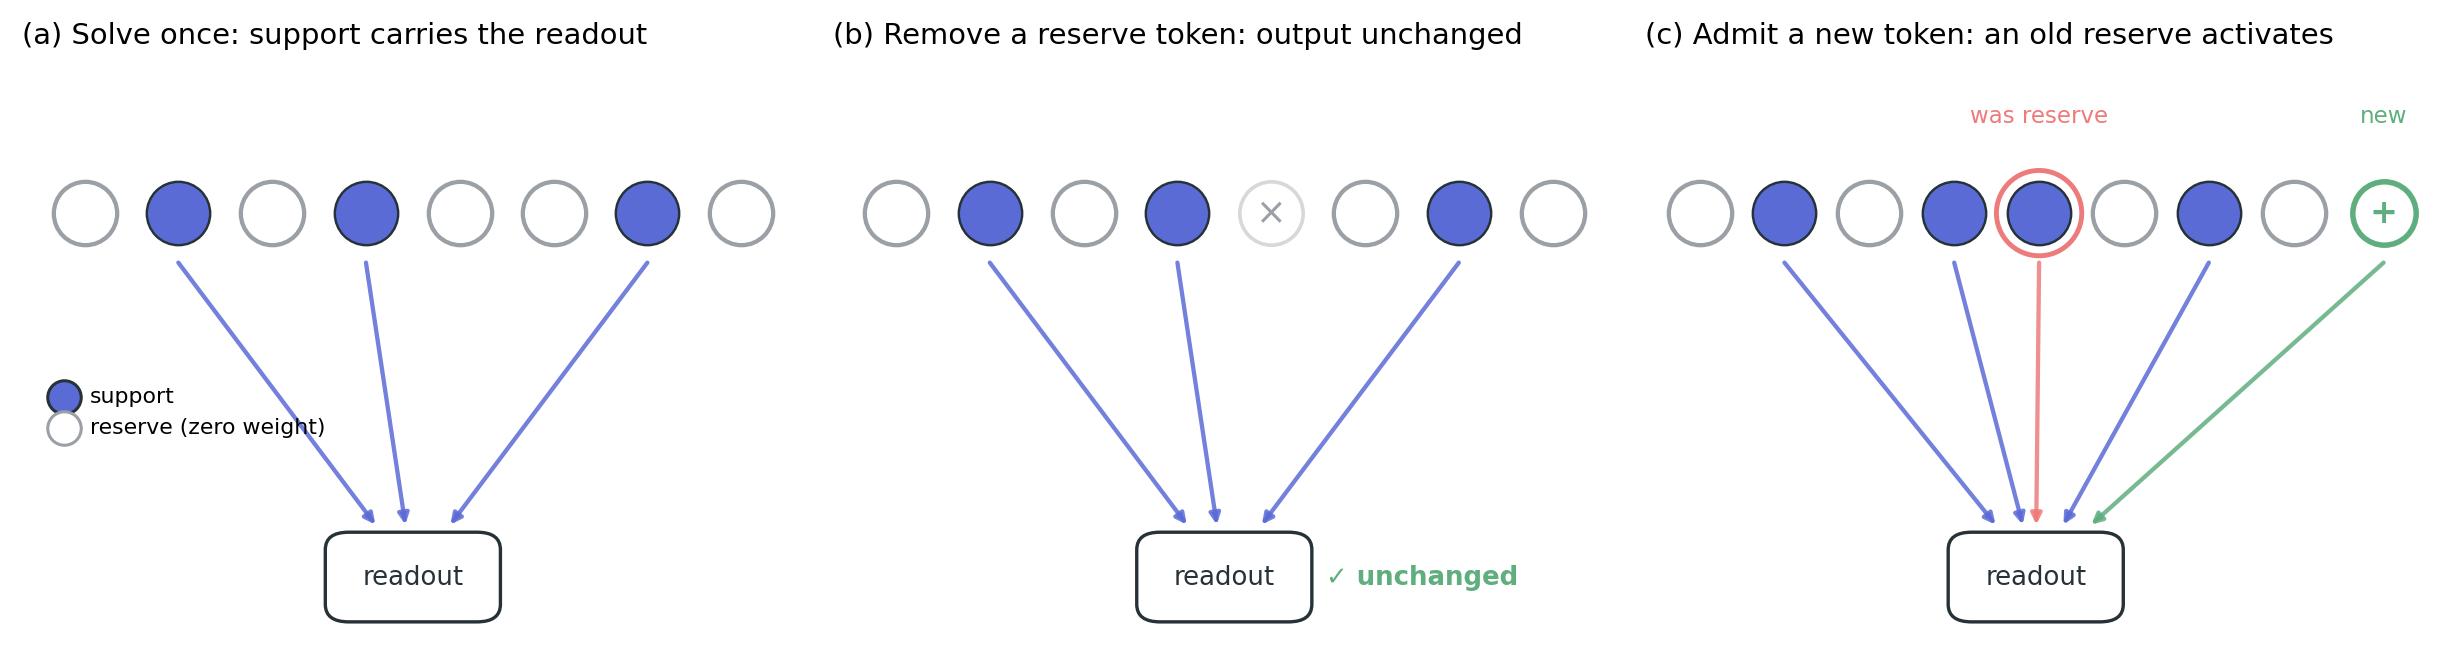
\includegraphics[width=\linewidth]{figs/hero_contract.png}
\caption{\emph{A point-in-time certificate and its sharp boundary.}
Proposition~\ref{prop:reserve} certifies that removing a reserve token leaves
the solved readout unchanged; the implementation residual in
Example~\ref{ex:future} is \(4.6\times10^{-9}\). A later admission gives that
old reserve point coefficient \(0.033\), and the previously pruned state differs
from the full-history solve by \(4.1\times10^{-3}\) over the declared decision
probes. This construction proves Proposition~\ref{prop:not-future}.}
\label{fig:contract}
\end{figure}

\section{Related Work}

\textbf{Test-time learning and recurrent memory.} Linear attention,
DeltaNet, the mesa layer, Titans, and selective state-space models treat
context processing as an online learning or recurrent-memory
problem~\citep{lina,fwp,deltanet,mesa,mesanet,titans,mamba}. These methods
compress history into dense online or recurrent state; they do not ordinarily
identify a token whose coefficient is exactly zero in a declared convex
problem, nor maintain the bordered inverse needed to compare a deletion with a
retained-key refit. SV-Attention contributes that audit interface: a named
reference problem, an inspectable active set, and operation-specific
certificates. This is a structural distinction, independent of whether those
architectures are better quality or faster in a particular workload.

\textbf{Cache selection.} H2O and SnapKV rank cache entries using measured
attention statistics~\citep{h2o,snapkv}. Their guarantees are empirical.
VeriCache preserves exact outputs by retaining a full reference cache for
verification~\citep{vericache}. SV-Attention instead certifies that a
zero-coefficient entry is inert for the current solved gate, but it does not
retain a full history and therefore does not inherit future equivalence after
continued admissions.

\textbf{Unlearning and differentiable optimization.} Exact machine
unlearning is commonly defined relative to retraining without the target
data~\citep{caoyang,unlearn}. ECO applies decremental SVM machinery to a
classifier head~\citep{eco}; we apply a fixed-\(C\) decrement to context memory.
OptNet and differentiable convex layers obtain gradients by differentiating KKT
systems~\citep{optnet,dcl}. The maintained C\&P path already stores the bordered
KKT inverse needed by its custom backward.

\section{Memory contract and method}\label{sec:method}

\subsection{The fixed-\(C\) support-vector gate}\label{sec:gate}

Given context keys \(x_i\in\mathbb{R}^d\), values
\(v_i\in\mathbb{R}^{d_v}\), and a query \(q\), the block readout is
\begin{equation}
o(q)=
\frac{\sum_i \alpha_i\kappa(q,x_i)v_i}
     {\sum_i \alpha_i\kappa(q,x_i)},\qquad
\kappa(a,b)=\exp(-\lVert a-b\rVert^2/\sigma^2).
\end{equation}
The coefficients solve support vector data description
\begin{equation}
\min_{\alpha}\;
\alpha^\top K\alpha-\operatorname{diag}(K)^\top\alpha
\quad\text{s.t.}\quad
\sum_i\alpha_i=1,\qquad 0\leq\alpha_i\leq C,
\label{eq:svdd}
\end{equation}
where \(K_{ij}=\kappa(x_i,x_j)\). The primitive hyperparameter is the
absolute box \(C\). When we report \(\nu\), we use it once to calibrate
\(C=1/(\nu n_0)\) at a declared reference size \(n_0\); deletion and refit do
not recompute \(C\) after the set size changes.

The KKT conditions partition the keys into a margin set
\(S=\{i:0<\alpha_i<C\}\), an error set \(E=\{i:\alpha_i=C\}\), and a reserve
set \(R=\{i:\alpha_i=0\}\).

\begin{proposition}[Point-in-time reserve certificate]\label{prop:reserve}
Let \(\alpha^\star\) solve Equation~\ref{eq:svdd} for a fixed context and fixed
\(C\). If \(\alpha^\star_j=0\), then evicting key \(j\) without re-solving
leaves the objective value and the normalized readout \(o(q)\) unchanged for
every query with nonzero denominator. The restricted coefficient vector is
also optimal for the retained-key problem.
\end{proposition}

\begin{proof}
Restricting \(\alpha^\star\) to the retained indices preserves the sum and box
constraints, and every objective term involving \(j\) vanishes because
\(\alpha^\star_j=0\). Conversely, any better retained-key solution could be
extended by a zero coefficient at \(j\), contradicting optimality of
\(\alpha^\star\). The numerator and denominator of the readout likewise lose
only a zero-weight term.
\end{proof}

This exact-arithmetic statement applies to the solved state. The implementation
classifies reserve coefficients at a declared tolerance and logs the realized
readout residual separately.

\setlength{\fboxsep}{5pt}
\noindent\fbox{\begin{minipage}{0.96\linewidth}
\small
\refstepcounter{example}\label{ex:future}
\textbf{Example \theexample{} (Future activation after reserve removal).}
Use RBF keys \((-1,0),(1,0),(0,0.9)\), box \(C=1\), and kernel width
\(\sigma=5\). The third key is reserve. For query \(q=(0.25,0.1)\) and scalar
values \((1,2,9)\), removing it gives current decision-function deviation below
\(10^{-12}\) and attention-readout deviation
\(4.57099\times10^{-9}\). After admitting \((0,-10)\), the full-history solve
assigns the old reserve key coefficient \(0.03327001\); the maximum
full-history/pruned decision-function difference over the three original keys
and the admitted key is \(4.07857\times10^{-3}\).
\end{minipage}}

\begin{proposition}[No unconditional future-equivalence guarantee from reserve
status alone]
\label{prop:not-future}
Membership in the reserve set of the current solved problem is insufficient to
guarantee equivalence between a previously pruned state and the full-history
solve after arbitrary future admissions.
\end{proposition}

\begin{proof}
Example~\ref{ex:future} is a counterexample: the same key has zero coefficient
before the admission and positive coefficient afterward, and the two decision
functions then differ.
\end{proof}

Thus a future-safe result requires additional restrictions on admissions or
geometry, or enough retained information to revisit earlier decisions.

\subsection{Fixed-\(C\) decrement and refit target}\label{sec:increment}

For active-token deletion, the C\&P reverse path drives the target coefficient
to zero while preserving the KKT conditions and updating
\(\mathcal{R}=M^{-1}\), where
\begin{equation}
M=
\begin{bmatrix}
0 & \mathbf{1}^\top\\
\mathbf{1} & 2K_{SS}
\end{bmatrix}.
\end{equation}

\begin{proposition}[Fixed-\(C\) decrement target]\label{prop:decrement}
Assume the retained-key QP has a unique coefficient optimum. If the exact C\&P
reverse path completes while maintaining the KKT conditions and drives the
deleted coefficient to zero, its restricted coefficient vector equals a fresh
retained-key solution of Equation~\ref{eq:svdd} under the same \(C\).
\end{proposition}

\begin{proof}
At completion, removing the zero target coefficient leaves a retained-key state
that satisfies the primal, dual, and complementarity KKT conditions under the
unchanged box \(C\). These conditions are sufficient for the convex quadratic
program, and uniqueness identifies the coefficient vector with the fresh
refit.
\end{proof}

When the retained KKT solution also fixes the dual offset \(\rho\), the full
decision state coincides. With non-unique duplicate solutions, raw
coefficients and active partitions may differ while the decision function
\[
f(x)=2\sum_i\alpha_i\kappa(x,x_i)-\rho
\]
agrees. We therefore treat finite-probe decision-function deviation as the
primary duplicate-invariant metric and report numerical coverage separately.

\subsection{The two numerical paths}\label{sec:method-solver}

\begin{figure}[t]
\centering
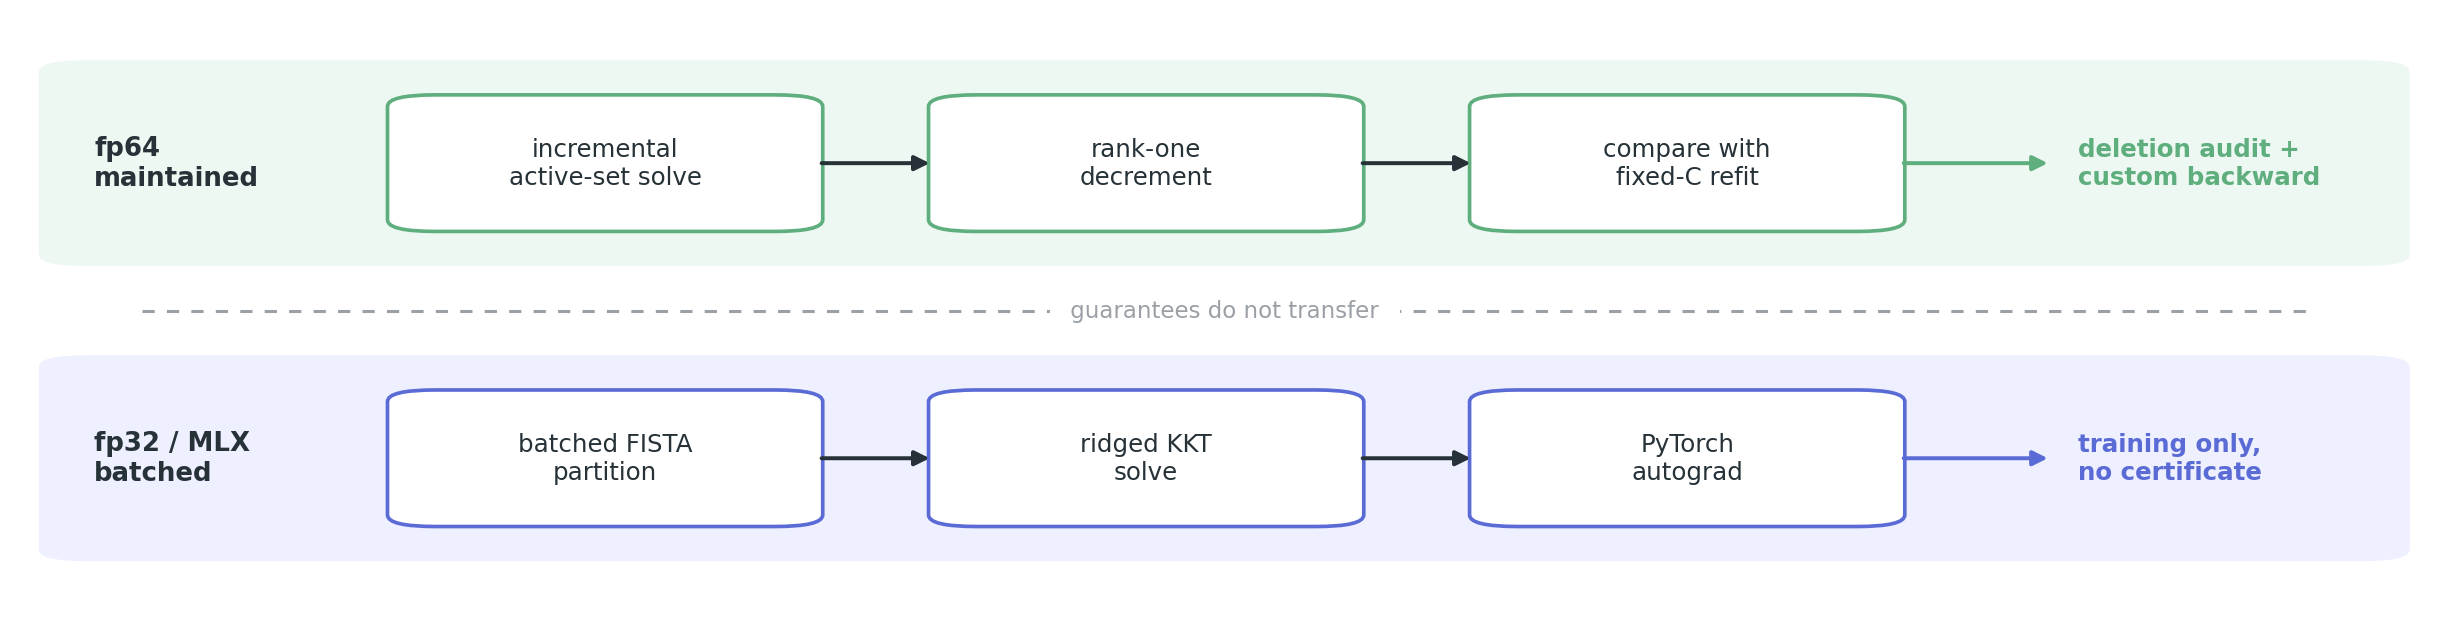
\includegraphics[width=\linewidth]{figs/two_numerical_paths.png}
\caption{\emph{A reusable separation of verification and training arithmetic.}
The fp64 maintained path supports the decrement/refit audit and custom
inverse-reusing backward. The batched FISTA/ridged-KKT path trades that
structure for parallel differentiable training. Claims attach to the path that
earns them.}
\label{fig:paths}
\end{figure}

\paragraph{Maintained verification path.}
The fp64 active-set implementation updates the bordered inverse through
rank-one operations and periodically refactors it. Within a fixed partition,
the custom vector--Jacobian product multiplies by
\(\mathcal{R}^{\top}\); it performs no second system solve
(Appendix~\ref{app:vjp}). ``Exact'' refers to the algebraic fixed-\(C\) target.
Every implementation claim is accompanied by measured coverage and tolerance.

\paragraph{Stabilized training path.}
For each sequence, head, and chunk, a batched single-precision FISTA solve
estimates the partition. PyTorch then solves a \(10^{-3}\)-ridged packed KKT
system and differentiates it with autograd
(Appendix~\ref{app:solver}). These coefficients are an approximation to
Equation~\ref{eq:svdd}. This path is trainable, but it is not the maintained
solver, does not reuse its inverse, and supplies no deletion certificate.

The separation in Figure~\ref{fig:paths} is deliberate. Verification favors a
maintained, inspectable fp64 state; training favors batched accelerator
operations. A trained model can still be audited by freezing its keys and
re-solving those keys on the maintained path.

\subsection{Causal usability probe}\label{sec:method-hybrid}

The causal layer freezes the long-range gate at chunk boundaries and adds a
dense local path so current queries can see recent tokens. The hybrid was
introduced only to test whether the memory can participate in end-to-end
training. Its local path is ordinary softmax and has no support-vector
certificate. Continued reserve pruning is point-in-time output-preserving at
each pruning event, but the resulting trajectory is not certified equivalent
to a never-pruned full-history solve.

\begin{table}[t]
\centering
\footnotesize
\caption{\emph{Contract card.} Each claim names its reference state and
arithmetic path; algebraic and empirical statements are kept distinct.}
\label{tab:contract}
\begin{tabular}{@{}
>{\raggedright\arraybackslash}p{0.13\linewidth}
>{\raggedright\arraybackslash}p{0.27\linewidth}
>{\raggedright\arraybackslash}p{0.23\linewidth}
>{\raggedright\arraybackslash}p{0.24\linewidth}@{}}
\toprule
operation & certified statement & reference and path & explicit boundary \\
\midrule
reserve removal &
the solved readout is unchanged when an algebraic zero-weight key is removed
without re-solving &
current fixed-\(C\) state; exact argument with logged fp64 residual &
no equivalence claim after arbitrary future admissions \\
\addlinespace
active deletion &
a completed exact decrement reaches the retained-key coefficient optimum under uniqueness &
fresh retained-key refit at the same \(C\); maintained fp64 path &
not a changed-\(C\) refit, re-contextualization, or deletion from model weights \\
\addlinespace
streaming pruning &
each reserve removal has a point-in-time certificate &
empirical bounded-memory trajectory after subsequent admissions &
not certified equal to a never-pruned full-history trajectory \\
\addlinespace
batched training &
autograd differentiates the ridged packed KKT system conditional on estimated masks &
fp32 FISTA masks plus \(10^{-3}\)-ridged solve &
no decrement or inverse-reuse guarantee; frozen keys require fp64 re-solving \\
\bottomrule
\end{tabular}
\end{table}

\section{Fixed-\(C\) deletion verification}\label{sec:forget}

We compare decrement with a fresh retained-key refit under identical \(C\) on
four regimes: Gaussian keys, redundant near-duplicates, real hourly MIMIC-IV
vitals, and keys produced by a trained recall model. Each of the \(300\)
attempted trials per regime removes two points and probes retained, removed,
and jittered locations. Figure~\ref{fig:deletion} and
Table~\ref{tab:deletion} report coverage before accuracy.

\begin{figure}[t]
\centering
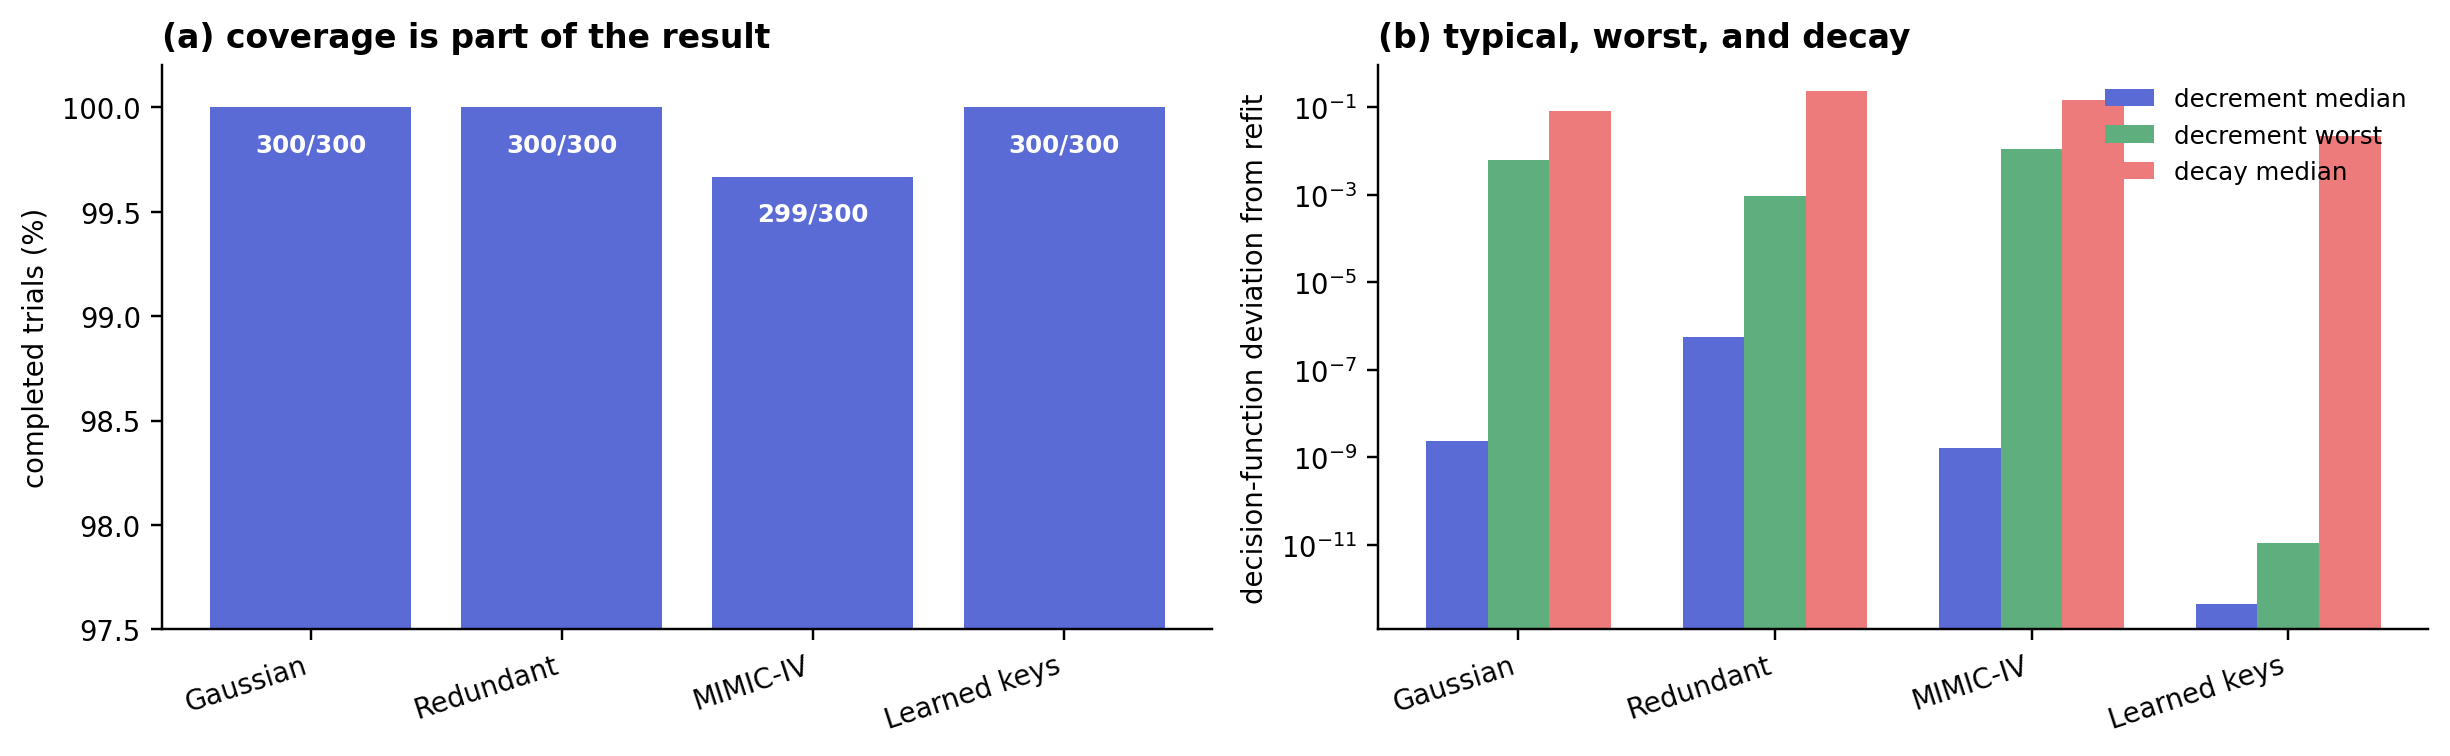
\includegraphics[width=\linewidth]{figs/deletion_evidence_v2.png}
\caption{\emph{Numerical coverage and agreement with the fixed-\(C\) refit.}
\emph{(a)} \(1{,}199/1{,}200\) attempted trials complete; the uncovered case is
a margin-empty decrement on MIMIC-IV. \emph{(b)} Median and worst
finite-probe decision-function deviation are shown separately. The largest
completed-trial deviation is \(1.1\times10^{-2}\) in the MIMIC-IV regime;
learned keys remain near \(10^{-12}\). Coefficient decay is evaluated against
the same refit.}
\label{fig:deletion}
\end{figure}

\begin{table}[t]
\centering
\small
\caption{Fixed-\(C\) decrement/refit audit. ``Part.'' is active-partition
agreement. Ill-conditioned near-duplicate problems can yield different
numerical partitions, so the redundant row's \(52\%\) does not by itself imply
functional failure; its median finite-probe decision-function deviation is
\(5.7\times10^{-7}\). Deviations are median / mean / worst over completed
trials.}
\label{tab:deletion}
\begin{tabular}{lccc}
\toprule
regime & coverage & part. & decision-function deviation \\
\midrule
Gaussian & \(300/300\) & \(99\%\) &
\(2.4\mathrm{e}{-9}/3.1\mathrm{e}{-5}/6.4\mathrm{e}{-3}\)\\
redundant & \(300/300\) & \(52\%\) &
\(5.7\mathrm{e}{-7}/3.1\mathrm{e}{-5}/9.6\mathrm{e}{-4}\)\\
MIMIC-IV & \(299/300\) & \(98\%\) &
\(1.6\mathrm{e}{-9}/5.6\mathrm{e}{-5}/1.1\mathrm{e}{-2}\)\\
learned keys & \(300/300\) & \(100\%\) &
\(4.5\mathrm{e}{-13}/9.7\mathrm{e}{-13}/1.1\mathrm{e}{-11}\)\\
\bottomrule
\end{tabular}
\end{table}

The single uncovered trial hits the implementation's explicit
margin-set-empty path. It is classified as an edge case, not removed from the
denominator. The redundant regime illustrates why partition equality is a
diagnostic rather than the equivalence criterion: exact partition agreement is
\(52\%\), while the median of the per-trial finite-probe maximum deviations is
\(5.7\times10^{-7}\). Ill-conditioned near-duplicate Gram matrices can yield
numerically fragile active-set walks and different numerical partitions. The
worst-case column keeps the finite-precision tail visible without assigning it
to a single cause. Coefficient decay, measured against the same refit, has
median deviation \(2.2\times10^{-2}\) to \(2.4\times10^{-1}\).

\paragraph{Deletion cost and concrete records.}
Across \(30\) uniform-random token removals at each
\(n\in\{120,256,384,512\}\), per-size median maintained-deletion latency is
\(0.30\)--\(1.04\) ms on the reference CPU, and the median per-trial
refit/deletion ratio is \(24\)--\(223\times\); timing is hardware-specific. On
frozen learned keys, deleting one fact leaves the other seven facts answerable,
and remove--add corrects one binding. On MIMIC-IV records, the completed
fixed-\(C\) path removes the selected patient's gate weight while retaining the
others. These are decision/readout audits, not a formal privacy guarantee or
deletion from model weights.

\section{Selection helps under a declared regime}\label{sec:selection}

The gate is a one-class boundary estimator, not a universal importance score.
Its selection bias is useful when informative tokens are atypical or when
context contains dense duplicates. We isolate the selection policy by giving
each method the same uniform-RBF readout and the same token budget.

\begin{figure}[t]
\centering
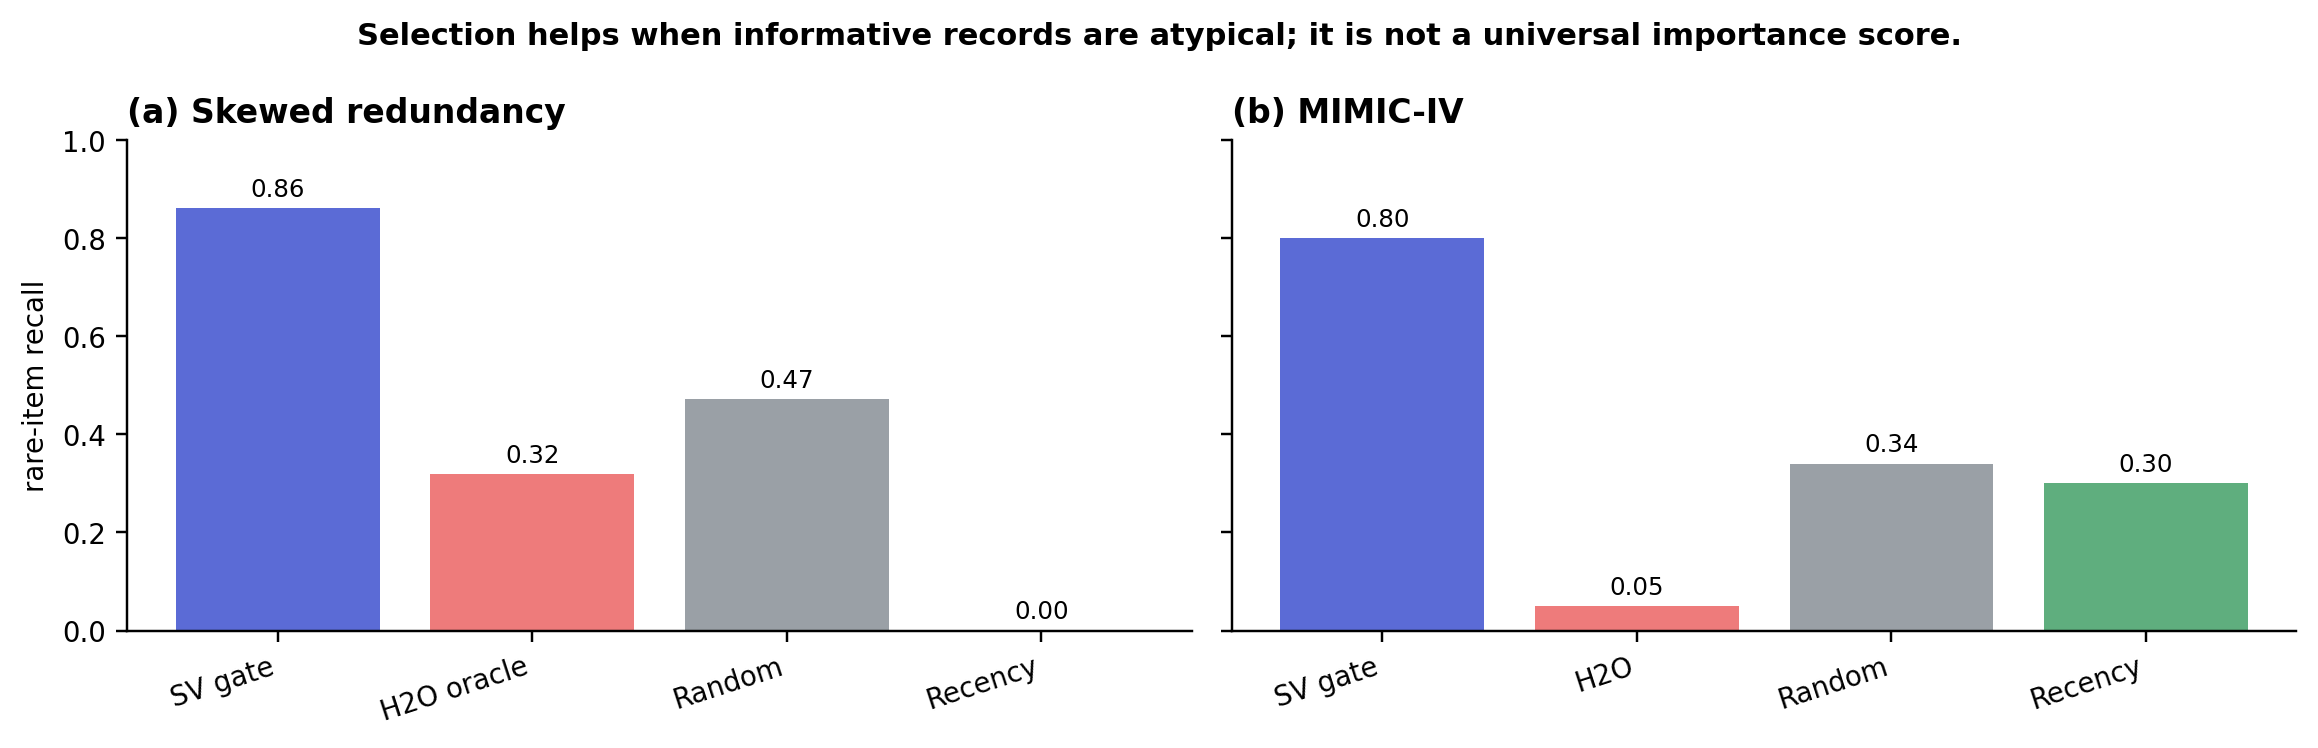
\includegraphics[width=0.94\linewidth]{figs/selection_scope_v2.png}
\caption{\emph{The selection advantage is regime-specific.}
\emph{(a)} Under skewed redundancy, support-set selection improves held-out
rare-group query recall relative to an oracle H2O-style RBF-mass selector that
sees the evaluation queries. \emph{(b)} On real ICU streams, atypical
deterioration hours align with the support boundary. The threshold label shares
five physiological channels with the six-channel gate, so this panel is a
retention-mechanics probe rather than independent predictive evidence.}
\label{fig:selection}
\end{figure}

\paragraph{Skewed redundancy.}
Contexts contain six singleton groups and six groups of ten near-duplicates.
At the gate's matched \(56\%\) budget, mean held-out singleton-group query
recall is \(0.861\), versus \(0.319\) for an oracle H2O-style RBF-mass selector
that sees the evaluation queries, \(0.472\) for random selection, and \(0\) for
recency. The support-vector policy itself is query-independent. This is a
fixed-context selection result; after continued admissions, the pruned
trajectory is evaluated empirically rather than certified against full history.

\paragraph{Real ICU streams.}
This experiment is designed to test retention mechanics: the threshold label
shares five physiological channels with the gate's six standardized inputs.
The MIMIC-IV cohort contains \(1{,}465\) eligible stays and \(222{,}935\)
hourly tokens; the retention analysis uses the \(1{,}329\) stays containing at
least one threshold-defined deterioration hour. At the support-defined mean
\(33\%\) per-stay budget, mean per-stay threshold-hour retention is \(0.80\)
for the support set versus \(0.05\) for the H2O-style self-RBF-mass selector.
The magnitude is therefore mechanistically expected, not independent clinical
prediction. We therefore add a held-out-channel control: events are defined by
unstandardized hourly SpO\(_2\), after within-stay filling and cohort-median
imputation, thresholded below \(90\); SpO\(_2\) is removed from every selector's
input. Across the \(718\) stays containing such an event, at a matched mean
\(32\%\) budget, support selection retains \(0.464\) of event hours versus
\(0.225\) for the H2O-style selector (recency \(0.409\); random \(0.333\)).
The paired mean difference is \(0.239\) (95\% stay-level percentile bootstrap
interval \(0.194\)--\(0.284\), \(10{,}000\) resamples, treating stays as
independent resampling units). This control removes direct label-channel reuse
while preserving the same selection protocol. A separate next-six-hour
prediction task provides the downstream control: SV-Attention reaches AUROC
\(0.696\), below the LSTM \(0.783\) and softmax \(0.751\). Selection that
preserves atypical hours does not by itself optimize local trend prediction.

\paragraph{\textbf{Negative control---the gate does not explain distinct-key
recall.}}
On ten-pair distinct-key recall, the ungated RBF readout reaches \(0.970\)
recall@1 versus \(0.955\) with the max-margin gate, whose support fraction is
\(1.00\). Every key is therefore active: the gate performs no token selection
in this regime, which explains why turning it off does not hurt. The useful
component is the distance-kernel readout. This ablation prevents us from
attributing clean retrieval gains to the gate. Our positive selection evidence
is confined to the evaluated redundancy and atypicality probes in
Figure~\ref{fig:selection}.

\section{Trainability and language-model usability}\label{sec:trainable}

\subsection{Gradient and solver checks}\label{sec:grad}

The maintained custom backward matches finite differences for coefficients,
decision scores, and the complete readout. A student layer reduces
teacher-matching loss by \(99\%\) in \(200\) steps. The batched ridged path also
passes end-to-end gradient checks, but that result validates the approximation
it actually differentiates, not the unregularized fp64 coefficients.

\subsection{Throughput boundary}\label{sec:throughput}

At the \(3.22\)M-parameter configuration, the mixed PyTorch--MLX training path
reaches \(9{,}125\) tokens/s on an Apple M3 Ultra, \(35.8\times\) slower than
the repository's unfused MPS softmax. The CPU softmax diagnostic is also
\(6.1\times\) faster. Exact active-set inference is slower still. These measurements
establish that small experiments are feasible; they do not establish a
competitive architecture or accelerator kernel.

\subsection{Language modeling is a bounded probe}\label{sec:quality}

At \(3.22\)M parameters on a \(5\)M-byte enwik8 prefix, all seven paired seeds
favor the hybrid: mean best-validation BPC is \(2.178\) versus \(2.383\) for a
token-budget-matched sliding-window Transformer. The mean paired relative
improvement is \(8.6\%\), and a two-sided paired test on absolute BPC
differences gives \(p=0.001\). On TinyStories, the hybrid is lower on all three
seeds, a directionally positive but non-significant result (\(p=0.057\)).

At matched \(6{,}000\)-step budgets, the larger-scale comparison reverses. At
\(10\)M parameters and five seeds, the hybrid is \(2.5\%\) worse on average
with high between-seed variation; one \(32\)M run is substantially behind.
The traces are consistent with slower and less stable gate optimization, but
they do not match models at convergence. Whether the comparison changes at
matched convergence remains open. Thus the small-scale result establishes
trainability, while the larger runs identify an optimization problem rather
than a scale-level quality verdict.

\section{Discussion and limitations}\label{sec:limitations}

The central result is an operational memory contract. A constrained test-time
memory exposes zero coefficients and an algebraically reversible fixed-\(C\)
solve, enabling point-in-time selection and retained-refit deletion statements
that an undifferentiated dense state does not expose. Their conditions are:

\begin{itemize}
\item \textbf{Selection is point-in-time.} Removing a current reserve token
preserves the exact solve's current readout; implementation residual is
tolerance-bounded. Future admissions can activate that token in the full-history
solve, so bounded streaming is an empirical pruned trajectory.
\item \textbf{Deletion is relative to fixed \(C\) and retained keys.} Changing
\(C\), contextualizing neighbors again, or deleting from pretrained weights
defines a different reference problem.
\item \textbf{The implementation is numerical.} \(1{,}199/1{,}200\) audited
trials complete; completed-trial deviations include a visible
\(1.1\times10^{-2}\) worst case. The margin-empty path needs a production
implementation or explicit refit fallback.
\item \textbf{Training and verification use different solvers.} The batched
path is approximate and does not inherit fp64 deletion or inverse-reuse claims.
\item \textbf{Current performance has a measured boundary.} The present path is
much slower than softmax, trails the ICU prediction baselines, and has no
confirmed language-model advantage beyond small scale.
\item \textbf{The threat model is narrow.} We measure state,
decision-function, and readout agreement, not membership inference, prior
snapshots, or legal compliance.
\end{itemize}

These limitations change how the system should be used. A fixed-context memory
can expose an auditable current support set and a verified deletion path. A
production streaming system must either retain enough information to revisit
future active sets, accept an empirical pruning policy, or derive a stronger
future-safe certificate under additional assumptions.

\section{Conclusion}

SV-Attention turns active-set structure into an auditable memory interface.
Reserve coefficients provide a proved point-in-time removal certificate, and a
named counterexample proves that current reserve status alone does not
guarantee full-history equivalence for every future admission sequence.
Active-token decrement has an explicit algebraic target---the fixed-\(C\)
retained-key refit---and the fp64 implementation completes
\(1{,}199/1{,}200\) audited trials with its numerical distribution reported. A
separate batched path demonstrates that the mechanism can be trained without
conflating training arithmetic with verification arithmetic. Our positive
selection evidence is confined to the evaluated redundancy and ICU
atypicality probes. Within that scope, the results give an operator a concrete
answer to what was solved, what can be removed now, and what reference state
deletion matches.

\section*{Data Availability and Reproducibility}

Source and reproducibility materials accompany this preprint at
\url{https://github.com/VyLabs-AI/sv-attention}.
All synthetic experiments, solvers, tests, figure scripts, and aggregate
evidence files are released with fixed seeds. MIMIC-IV v3.1 is available only
to credentialed PhysioNet users under its data use agreement; we release
preprocessing and experiment code but no source record or derived cache. The
v2 package includes a claim-to-command map, dependency tiers, hardware notes,
and a generator for the four claim-boundary figures. The headline checks use:
\begingroup
\small
\begin{verbatim}
python -m pytest tests/test_fast_solver.py -q
python -m clinical_seq.e2_selection \
  --held-out-vital spo2 --max-stays 1465
\end{verbatim}
\endgroup
Every deletion report records attempted and completed counts, failure reasons,
fixed \(C\), and numerical distributions.
